\renewcommand{\theequation}{\theenumi}
\begin{enumerate}[label=\arabic*.,ref=\thesubsubsection.\theenumi]
\numberwithin{equation}{enumi}
\item \textbf{Proof} For a general polynomial equation of degree 2,
\\
$p(x,y) \implies Ax^2+Bxy+Cy^2+Dx+Ey+F=0$
\\
The vector form is 
\begin{align}
\label{eq:vector_form}
\vec{x}^T \myvec{A & B/2\\B/2 & C}\vec{x}+ \myvec{D & E}\vec{x}+F=0
\end{align}
\item For eq: $ y = x^2 - 1$
\\
Vector form is given by
\begin{align}
\vec{x}^T \myvec{1 & 0\\0 & 0}\vec{x}+\myvec{0 & -1}\vec{x}-1=0
\end{align}
(From the equation \ref{eq:vector_form}.)
\\
Thus,
\begin{align}
y=0
\\
\implies x^2-1=0
\\
x=+1,-1
\end{align}
Hence +1,-1 are zeros, which can be verified from the figure \ref{fig:parab1}
\begin{figure}[!ht]
\includegraphics[width=\columnwidth]{./figs/conics/parabola1.eps}
\caption{Parabola 1}
\label{fig:parab1}
\end{figure}
\item For eq: $ y = \brak{x+1} \brak{x-2}$
\\
Equation can be represented as
\\
$y=x^2-x-2$
\\
Vector form is given by
\begin{align}
\vec{x}^T \myvec{1 & 0\\0 & 0}\vec{x}+\myvec{-1 & -2}\vec{x}-2=0
\end{align}
(From the equation \ref{eq:vector_form}.)
\\
Thus,
\begin{align}
y=0
\\
\implies \brak{x+1} \brak{x-2}=0
\\
x=-1,+2
\end{align}
Hence -1,+2 are zeros, which can be verified from the figure \ref{fig:parab2}
\begin{figure}[!ht]
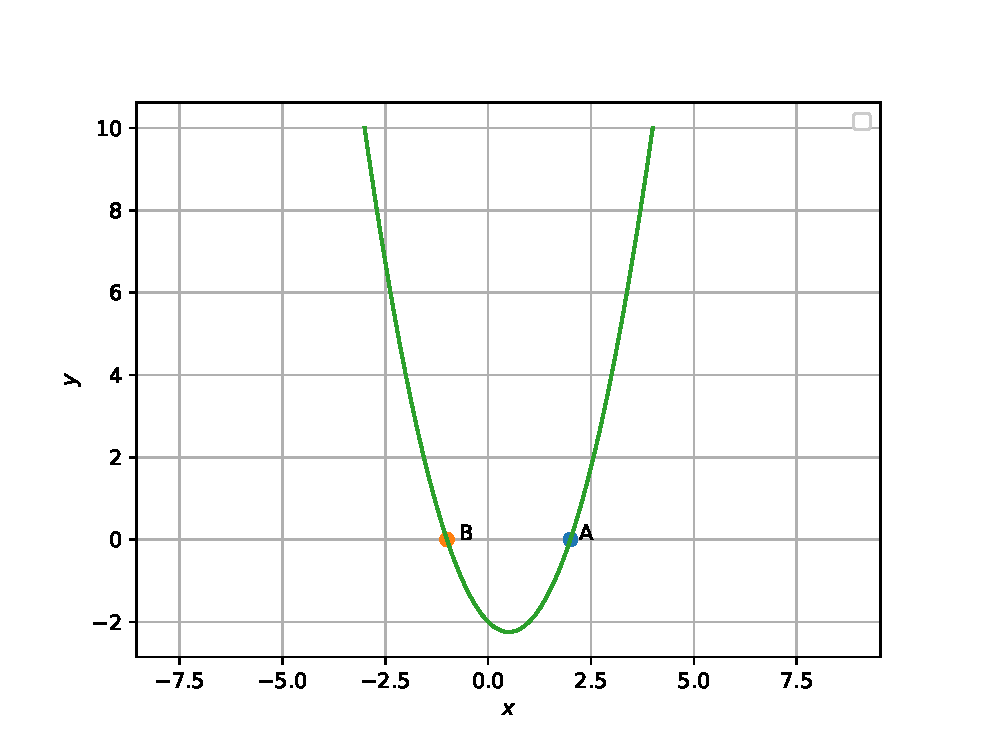
\includegraphics[width=\columnwidth]{./figs/conics/parabola2.eps}
\caption{Parabola 2}
\label{fig:parab2}
\end{figure}
\item For eq: $ y = x^2$
\\
Vector form is given by
\begin{align}
\vec{x}^T \myvec{1 & 0\\0 & 0}\vec{x}+\myvec{0 & -1}\vec{x}=0
\end{align}
(From the equation \ref{eq:vector_form}.)
\\
Thus,
\begin{align}
y=0
\\
\implies x^2=0
\\
x=0
\end{align}
Hence 0 is the  zero, which can be verified from the figure \ref{fig:parab3}
\begin{figure}[!ht]
\includegraphics[width=\columnwidth]{./figs/conics/parabola3.eps}
\caption{Parabola 3}
\label{fig:parab3}
\end{figure}
\item For eq: $ y = 3x^2-1$
\\
Vector form is given by
\begin{align}
\vec{x}^T \myvec{3 & 0\\0 & 0}\vec{x}+\myvec{0 & -1}\vec{x}-1=0
\end{align}
(From the equation \ref{eq:vector_form}.)
\\
Thus,
\begin{align}
y=0
\\
\implies 3x^2-1=0
\\
x=+\frac{1}{\sqrt{3}},-\frac{1}{\sqrt{3}}
\end{align}
Hence $\frac{1}{\sqrt{3}},-\frac{1}{\sqrt{3}} $are the  zeros, which can be verified from the figure \ref{fig:parab4}
\begin{figure}[!ht]
\includegraphics[width=\columnwidth]{./figs/conics/parabola4.eps}
\caption{Parabola 4}
\label{fig:parab4}
\end{figure}


\end{enumerate}